\chapter{EPPSETIN'S \greedyAlgo\ ALGORITHM}
\label{sec:greedy}

The \greedyAlgo\ algorithm is one of the fastest algorithms among the reset word generation heuristics in the literature. The correctness of the algorithm is based on the following proposition (see Theorem 1.14 in the book \cite{Broy05}, \cite{Starke1972}).

\begin{proposition}
	\label{prop:synchronizable}
	An automaton ${\cal A}=(S,\Sigma,\delta)$ is synchronizing iff $\forall s_i,s_j \in S$, there exists a merging sequence for $\{ s_i, s_j \}$.
\end{proposition}

\noindent \greedyAlgo\  uses the shortest merging sequences of pairs to find a short reset word. Like most of the algorithms mentioned in Section \ref{sec:Intro}, \greedyAlgo\ has two  phases. In the first phase, it finds the shortest merging sequences for all pairs. If there is a pair which is not mergeable, due to Proposition~\ref{prop:synchronizable}, the automaton is not synchronizing. Otherwise, the algorithm continues with the second phase.

The merging sequences of pairs are stored in a function $\tau : S^{\langle 2 \rangle} \rightarrow \Sigma^\star$, which is called the \textit{pairwise merging function} (PMF) for ${\cal A}$. If $\{ s_i, s_j \}$ is mergeable, then $\tau(\{ s_i, s_j \})$ is the merging sequence, otherwise it is undefined. Note that PMF does not have to be unique, i.e., $\tau(\{ s_i, s_j \})$ may differ, however  $|\tau(\{ s_i, s_j \})|$ is unique and the shortest possible. To find all the shortest merging sequences, a breadth first search (BFS) can be initiated over the pair automata. By using the inverse of transition function and starting from $\{ s_i, s_i \}$ singletons, all mergeable pairs and their shortest merging sequences can be found. Let $p=|\Sigma|$ and $n=|S|$; in worst case, the algorithm traverses all edges, i.e., $p$ letters of each $n(n-1)$ pairs and $n$ singletons should be checked. Therefore the complexity of the first phase is $O(pn^2)$. 

\pagebreak

Algorithm \ref{algo:BFS} keeps track of most recently computed mergeable pairs via a list, which is called \textit{frontier set} ($F$). The level of a frontier set refers to the length of the corresponding merging sequences inside. Since $\tau(\{ s_i, s_i \})=\epsilon$, singletons are placed in the root level, level 0, of BFS. The \textit{remaining set} ($R$) is the set of pairs whose merging sequences are not computed yet. At each iteration of Algorithm \ref{algo:BFS}, new frontier and remaining sets are computed for the next level. 


\begin{algorithm}[ht]
	\caption{Computing a PMF $\tau : S^{\langle 2 \rangle} \rightarrow \Sigma^\star$}
	\label{algo:BFS}
	\SetKwInOut{Input}{input}\SetKwInOut{Output}{output}
	\Input{An automaton ${\cal A}=(S,\Sigma,\delta)$}
	\Output{A PMF $\tau : S^{\langle 2 \rangle} \rightarrow \Sigma^\star$}
	
	%compute the reverse automaton ${A}^{-1} = (S,\Sigma,\delta^{-1})$ of $A$\;
	\lForEach{singleton $\{ s,s \} \in S^{\langle 2 \rangle}$}{$\tau(\{ s,s \}) = \varepsilon$}
	\lForEach{pair $\{ s_i,s_j \} \in S^{\langle 2 \rangle}$}{$\tau(\{ s_i,s_j \}) =$ {\em undefined}}
	
	$F \longleftarrow \{ \{ s,s \} | s \in S \}$; \tcp{all singletons of $S^{\langle 2 \rangle}$}
    $R \longleftarrow \{ \{ s_i, s_j \} | s_i,s_j \in S \wedge s_i \neq s_j \}$; \tcp{all pairs of $S^{\langle 2 \rangle}$}
	\While{$R$ is not empty and $F$ is not empty}
	{
		$F,R,\tau \longleftarrow \mbox{BFS\_step}(A,F,R,\tau)$\;
	}
\end{algorithm}

\begin{proposition}
	\label{prop:merging}
	Let $\{ s_i,s_j \}$ be a pair in $S^{\langle 2 \rangle}$. If $w \in \Sigma^*$ is a merging sequence for $\delta(\{ s_i,s_j \}, x)$ then $xw$ is a merging sequence for $\{s_i,s_j \}$.
\end{proposition}

Thanks to the inverse of transition function and Proposition \ref{prop:merging}, Algorithm \ref{algo:BFS-step-F2R} constructs PMF from the most recent frontier set. At lines 3-4, the algorithm searches the pairs which can reach the frontier set pairs by applying a single letter. When the algorithm finds such a pair whose merging sequence has not been defined yet, it marks the pair as the next frontier set's pair for the next iteration and sets its merging sequence. Since the algorithm computes the PMF of the remaining set by using the frontier set, it is called \textit{frontier to remaining} (F2R). 

\begin{algorithm}[ht]
	\caption{{BFS\_step (F2R)}}
	\label{algo:BFS-step-F2R}
	
	\SetKwInOut{Input}{input}\SetKwInOut{Output}{output}
	\Input{An automaton ${\cal A}=(S,\Sigma,\delta)$, the frontier $F$, the remaining set $R$, $\tau$}
	\Output{The new frontier $F'$, the new remaining set $R'$, and updated function $\tau$}
	
	$F' \longleftarrow \emptyset$\;
	\ForEach{$ \{ s_i,s_j \} \in F$}
	{
		\ForEach{$x \in \Sigma$}
		{
			\ForEach{$\{ s'_i,s'_j\}$ such that $s'_i \in \delta^{-1}(s_i,x)$ and $s'_j \in \delta^{-1}(s_j,x)$}
			{
				\If(\tcp*[h]{$\{ s'_i,s'_j\} \in R$}){$\tau(\{ s'_i,s'_j\})$ is undefined}
				{
					$\tau(\{ s'_i,s'_j \}) \longleftarrow x \tau(\{ s_i,s_j \})$\;
					$F' = F' \cup \{ \{ s'_i,s'_j \}  \} $\;
				}
			}
		}
	}
	let $R'$ be $R \setminus F'$;
\end{algorithm}

When the first phase is completed, Algorithm \ref{algo:greedy} first checks if the automaton is synchronizing or not in $O(n^2)$ (lines 2-3). It then initializes the \textit{set of active states} ($C$) as the set of all states and the initial reset word as empty. After that, iteratively, it selects the shortest merging sequence of all active pairs, appends it to reset word, and finally updates the set of active states by applying the selected merging sequence. This operation is repeated until only a single active state is left. 

\pagebreak

At each iteration, the merging sequence is applied, so the cardinality of $C$ decreases. Therefore, at most $n-1$ iterations are performed. At line 7, the algorithm finds the active pair with the shortest merging sequence which takes $O(n^2)$ per iteration. Line 8 takes constant time. The length of each merging sequence can be at most $n^2$. Therefore the time complexity of line 9 is $O(n^3)$ for a single iteration. Overall, the second phase takes $O(n^4)$ and Algorithm \ref{algo:greedy} requires $O(pn^2 + n^4)$ time. 

The upper bounds of the phases can be computed in a slightly different way. For a synchronizing automaton, the first phase is $\Omega(n^2)$ since it finds a merging sequence for all pairs. At best, phase two takes a merging sequence with length of one, which is also a reset word. Then the algorithm applies the merging sequence to all states. Therefore, the lower bound of the second phase is $\Omega(n)$. Thus Algorithm \ref{algo:greedy} has $O(pn^2 + n^4)$ and $\Omega(n^2)$ time complexity. Since there is a huge gap between the best  and the worst case complexities, we extended our observations with the empirical results. In the next subsection, the bottleneck of the algorithm is introduced with a thorough experimental analysis.

\begin{algorithm}[ht]
	\caption{Eppstein's \greedyAlgo\ algorithm}
	\label{algo:greedy}
	
	\SetKwInOut{Input}{input}\SetKwInOut{Output}{output}
	\Input{An automaton ${\cal A}=(S,\Sigma,\delta)$}
	\Output{A reset word $\Gamma$ for ${\cal A}$ (or fail if ${\cal A}$ is not synchronizable)}
	
	%{--- Phase 1 ---}
	compute a PMF $\tau$ using Algorithm~\ref{algo:BFS}\;
	\If{there exists a pair $\{ s_i,s_j \}$ such that  $\tau(\{ s_i,s_j \})$ is undefined}
	{
		report that ${\cal A}$ is not synchronizable and exit;	
	}

	
	%{--- Phase 2 ---}
	$C = S$; \tcp{$C$ will keep track of the current set of states}
	$\Gamma = \varepsilon$; \tcp{$\Gamma$ is the synchronizing sequence to be constructed}
	
	\While(\tcp*[h]{we have two or more states yet to be merged}){$|C| > 1$}
	{
		$\{ s_i,s_j \} = Find\_Min(C, \tau)$\;
		
		
		$\Gamma = \Gamma \; \tau(\{ s_i,s_j \})$\;
		$C = \delta(C,\tau(\{ s_i,s_j \}))$;
	}
\end{algorithm}


\begin{algorithm}[ht]
	\caption{Find\_Min}
	\label{algo:find-min}
	
	\SetKwInOut{Input}{input}\SetKwInOut{Output}{output}
	\Input{Current set of state $C$ and the PMF function $\tau$}
	\Output{A pair of states $\{ s_i,s_j \}$ with minimum $|\tau(\{ s_i,s_j \})|$ among all pairs in $C^{\langle 2 \rangle}$}
	
	$\{ s_i,s_j \} =$ undefined\;
	\ForEach{$ \{ s_k,s_\ell \} \in C^{\langle 2 \rangle}$}
	{
		\If{$\{ s_i,s_j \}$ is undefined or $|\tau(\{ s_k,s_\ell \})| < |\tau(\{ s_i,s_j \})|$}
		{
			$\{ s_i,s_j \} = \{ s_k, s_\ell \}$
		}
	}
\end{algorithm}



\section{Analysis on \greedyAlgo}
\label{sec:greedy-analysis}

As discussed in Section \ref{sec:greedy}, the time complexity of \greedyAlgo\ is $O(pn^2 + n^4)$. For most of the cases, $p$ is too small when compared to $n$. Hence, the complexity of the second phase, $O(n^4)$, dominates the first phase in theory. To analyze the algorithm, we performed experiments on 100 randomly generated automata for each  $p \in \{2, 8, 32, 128\}$ letters and  $n \in \{2000, 4000, 8000\}$ states. To generate a random automaton, for each state $s$ and input $x$, $\delta(s,x)$ is randomly assigned to a state $s' \in S$. In addition, we used \v{C}ern\'y automata~\cite{cerny} for $n \in \{2000, 4000, 8000\}$ states. All the experiments are excuted on a single machine running on 64 bit CentOS 6.5 equipped with 64GB RAM and a dual-socket Intel Xeon E7-4870 v2 clocked at 2.30 GHz where each socket  has 15 cores~(30 in total). In Table \ref{table:phase-comparison}, experiments from 1200 randomly generated automata show that the execution time of the second phase does not dominate the overall time of the algorithm for random automata.  

\begin{table}[ht]
	\center
	\scalebox{0.89}{
		\begin{tabular}{r|rrr|rrr|rrr}
		&\multicolumn{3}{|c}{$n = 2000$}&\multicolumn{3}{|c}{$n = 4000$}&\multicolumn{3}{|c}{$n = 8000$}\\
		$p$ & $t_{PMF}$ & $t_{ALL}$ & $\frac{t_{PMF}}{t_{ALL}}$ & $t_{PMF}$ & $t_{ALL}$ & $\frac{t_{PMF}}{t_{ALL}}$ & $t_{PMF}$ & $t_{ALL}$ & $\frac{t_{PMF}}{t_{ALL}}$\\\hline
			2		& 0.172	& 0.185	& 0.929	& 1.184		& 1.240		& 0.954	& 5.899		& 6.325		& 0.933 \\
			8		& 0.504	& 0.517	& 0.975	& 2.709		& 2.768		& 0.978	& 14.289	& 14.721	& 0.971 \\
			32		& 2.113	& 2.126	& 0.994	& 9.925		& 9.986		& 0.994	& 51.783	& 52.233	& 0.991 \\
			128		& 9.126	& 9.140	& 0.999	& 40.356	& 40.418	& 0.998	& 193.548	& 193.982	& 0.998 \\
			\v{C}ern\'y	& 0.096	& 4.836	& 0.020	& 1.026		& 42.771	& 0.024	& 5.584		& 797.692	& 0.007
		\end{tabular}
	}
	\caption{Sequential PMF construction time ($t_{PMF}$), and overall time ($t_{ALL}$) in seconds}
	\label{table:phase-comparison}
\end{table}

To understand the behavior of the algorithm, we extended our experiments by analyzing the structure of PMF. While computing time complexity of the algorithm, the length of the merging sequence is at most $n^2$. However, Table \ref{table:levels} shows that $n^2$ is loose bound for the length of merging sequence. For instance, when automata with 8000 states and 128 letters are considered, the lengths of merging sequences in PMF are at most 3, not 64000000. Another observation is that the second phase tends to pick shorter length of merging sequences. For example, when we take an automaton with 8000 states and 2 letters, the longest merging sequence in PMF has the length 16.9. The second phase uses only merging sequences with length 12.1 and less. Thus, the merging sequences of almost 30\% of the nodes are  unnecessarily computed (see Figure \ref{fig:nodes-at-levels}).

\begin{table}[ht]
	\center
	\begin{tabular}{r|rrr|rrr|rrr}
 		& \multicolumn{3}{c|}{n=2000} & \multicolumn{3}{c|}{n=4000} & \multicolumn{3}{c}{n=8000} \\
		p &  $h_{PMF}$ &  $h_{max}$ &  $h_{mean}$ &  $h_{PMF}$ &  $h_{max}$ &  $h_{mean}$ &  $h_{PMF}$ &  $h_{max}$ &  $h_{mean}$ \\ \hline
 		2 &  14.2 &  10.0 &  1.9 &  15.5 &  11.2 &  1.9 &  16.9 &  12.1 &  1.9 \\
 		8 &  5.0 &  4.0 &  1.3 &  6.0 &  4.2 &  1.3 &  6.0 &  4.6 &  1.3 \\
		32 &  3.1 &  2.7 &  1.1 &  4.0 &  2.9 &  1.1 &  4.0 &  3.0 &  1.1 \\
		128 &  3.0 &  2.0 &  1.0 &  3.0 &  2.0 &  1.0 &  3.0 &  2.1 &  1.0 \\
	\end{tabular}
	\caption{The length of the longest merging sequence in PMF($h_{PMF}$) constructed in the first phase for random automata; maximum ($h_{max}$), and average ($h_{mean}$) lengths for merging sequences, used in the second phase of Algorithm \ref{algo:greedy}.}
	\label{table:levels}
\end{table}


\begin{table}[ht]
	\center
	\begin{tabular}{r|rrr}
		n &  $h_{PMF}$ &  $h_{max}$ &  $h_{mean}$ \\ \hline
 		2000 & 1999000.0 & 1952000.0 & 8884.8 \\
 		4000 & 7998000.0 & 7808000.0 & 19750.8 \\
 		8000 & 31996000.0 & 31232000.0 & 43480.8
	\end{tabular}
	\caption{The length of the longest merging sequence in PMF($h_{PMF}$) constructed in the first phase for the \v{C}ern\'y automata; maximum ($h_{max}$), and average ($h_{mean}$) lengths for merging sequences, used in the second phase of \greedyAlgo .}
	\label{table:levels-cerny}
\end{table}

\begin{figure}[ht]
	\centering
	\subfigure[$p = 2$]{
		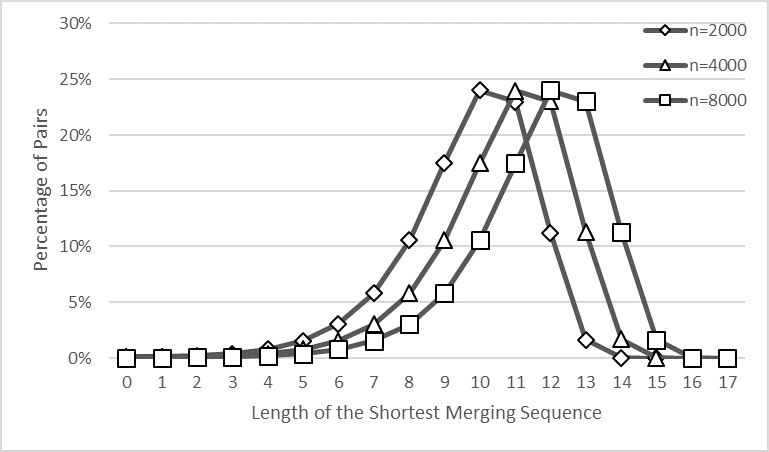
\includegraphics[width=0.47\textwidth]{figs/node_2.png}
	}
	\subfigure[$p = 8$]{
		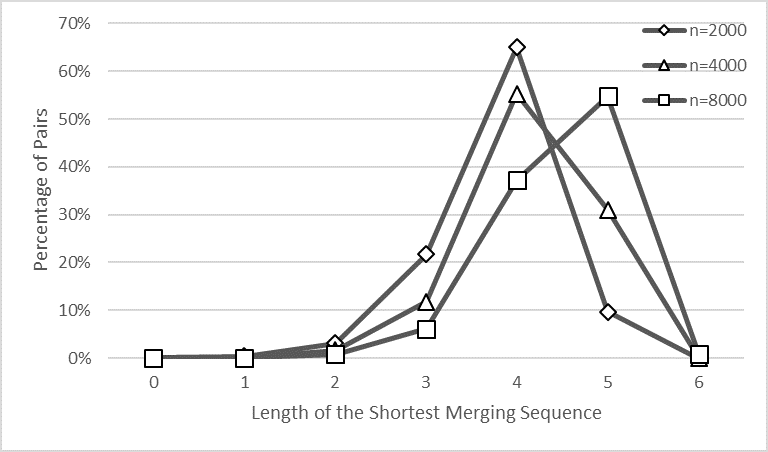
\includegraphics[width=0.47\textwidth]{figs/node_8.png}
	}
	\subfigure[$p = 32$]{
		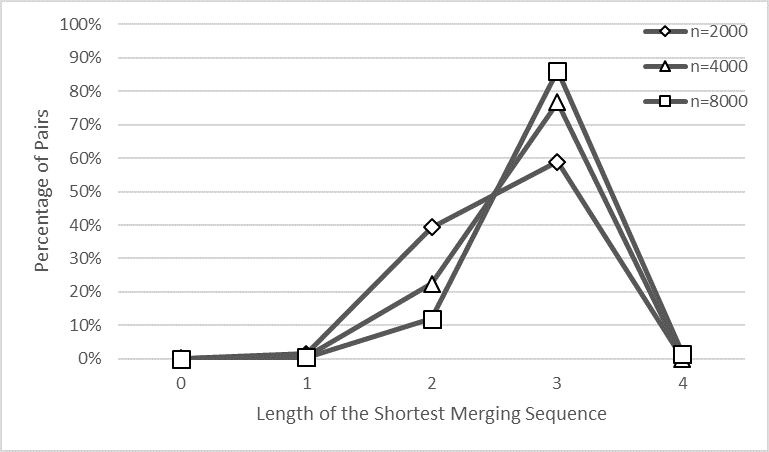
\includegraphics[width=0.47\textwidth]{figs/node_32.png}
	}
	\subfigure[$p = 128$]{
		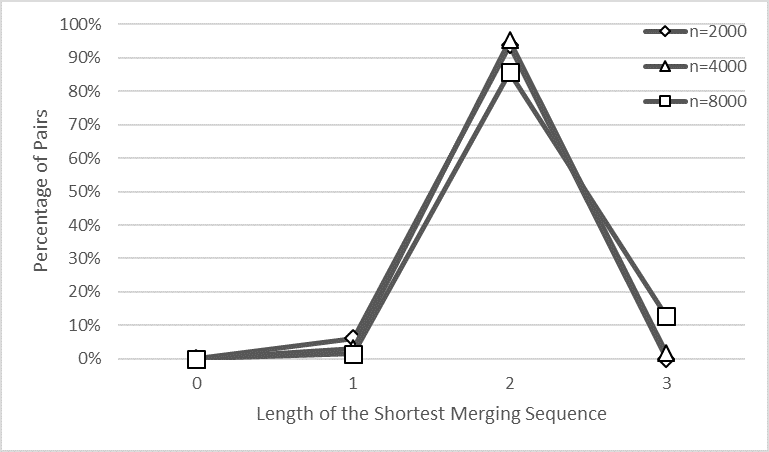
\includegraphics[width=0.47\textwidth]{figs/node_128.png}
	}
	\caption{The percentage of nodes at each level in PMF}
	\label{fig:nodes-at-levels}
\end{figure}

\pagebreak

With these experiments, we observed that the execution time of PMF construction phase in general dominates the \greedyAlgo\ algorithm except some special automata classes such as \v{C}ern\'y. Therefore, we focused on parallelization of PMF construction, which is explained in Section \ref{sec:parallel}. We also noticed that not all information from the first phase is used in the second phase. Based on these observations, various algorithmic improvements that make \greedyAlgo\  much faster are presented in Section \ref{sec:speedup}. But first, we will focus on its parallelization in the next section.

